\documentclass{article}
\usepackage[english]{babel}
\usepackage[margin=1in,rmargin=1in,includefoot]{geometry} 
\usepackage{blindtext}
\usepackage{everysel}
\usepackage{fancyhdr} 
\usepackage{graphicx} 
\usepackage{float}
\usepackage{physics}
\usepackage{textcomp}
\usepackage{algorithm}
\usepackage{verbatim}
\usepackage[noend]{algpseudocode}
\usepackage[none]{hyphenat} 
\usepackage{amsfonts} 
\usepackage{subcaption}
\usepackage{amsmath} 
\usepackage{mathtools}
\usepackage{indentfirst}
\usepackage{lipsum}
\usepackage{tgcursor}
\usepackage{IEEEtrantools}
\usepackage{cases}
\usepackage{xcolor}
\usepackage{hyperref}
\usepackage[T1]{fontenc}
\usepackage[utf8]{inputenc}
\usepackage{ragged2e}

\pagestyle{fancy}
\fancyhead{} 
\fancyfoot{} 
\fancyhead[L]{\slshape \MakeUppercase{Particle in a Box}}
\fancyhead[R]{\slshape Anwesh Bhattacharya}
\fancyfoot[C]{\thepage} 

\EverySelectfont{%
\fontdimen2\font=0.4em% interword space
\fontdimen3\font=0.2em% interword stretch
\fontdimen4\font=0.1em% interword shrink
\fontdimen7\font=0.1em% extra space
\hyphenchar\font=`\-% to allow hyphenation
}
\renewcommand{\baselinestretch}{1.5}

\newcommand{\psitilde}{\tilde{\psi}}
\newcommand{\psiN}{\psi_N}
\newcommand{\diffeq}{\textit{diffeq}}
\newcommand{\loss}{\textit{loss}}
\newcommand{\prob}{\textit{prob}}
\newcommand{\eigE}{\textit{eigen-energy}}
\newcommand{\NeuroDiffEq}{\textit{NeuroDiffEq} }
\newcommand{\MSE}{\textit{MSE}}
\newcommand{\iterations}{\textit{iterations} }
\newcommand{\eigenvalue}{\textit{eigenvalue} }
\newcommand{\probability}{\textit{probability} }
\newcommand{\nLratio}{$\displaystyle{\frac{n}{L}}$ }
\newcommand{\dmse}{$\displaystyle{\Delta \text{MSE}_{100}}$ }
\newcommand{\oom}[1]{$10^{#1}$}
\newcommand{\adam}{\texttt{\textbf{adam}} }
\newcommand{\callback}{\texttt{\textbf{callback}} }
\newcommand{\lTTTExit}{\texttt{\textbf{L3TExit}} }
\newcommand{\normalExit}{\texttt{\textbf{NormalExit}} }
\newcommand{\latexcomment}{}
\DeclarePairedDelimiter\ceil{\lceil}{\rceil}
\DeclarePairedDelimiter\floor{\lfloor}{\rfloor}


\setlength{\parskip}{1em}

\hypersetup{
    colorlinks=true,
    linkcolor=blue,
    filecolor=magenta,      
    urlcolor=cyan,
    pdftitle={Sharelatex Example},
}
\urlstyle{same}
\hypersetup{
    pdftitle={Using Neural Networks to Solve Schrodinger's Equation : Particle in a Box},
    pdfauthor={Anwesh Bhattacharya},
    pdfsubject={Quantum Mechanics},
    pdfkeywords={keyword1, keyword2},
    bookmarksnumbered=true,     
    bookmarksopen=true,         
    bookmarksopenlevel=1,       
    colorlinks=true,            
    pdfstartview=Fit,           
    pdfpagemode=UseOutlines,    % this is the option you were looking for
}

\begin{document}

%\hypersetup{linkcolor=black}
%\tableofcontents
%\hypersetup{linkcolor=blue}


\title{\textbf{Using Neural Networks to Solve Schrodinger's Equation : Particle in a Box}}
\author{Anwesh Bhattacharya}
\maketitle
\hrule

\section{Particle in a Box}

\justify
Time independent Schrodinger's equation is as follows -
$$\displaystyle{\frac{-\hbar^2}{2m} \dv[2]{\psi}{x}  + V(x)\psi(x) = E\psi(x)}$$


\justify
The potential for the system is as follows (\textit{L is the length of the box}) -
$$V(x) =
\left\{
	\begin{array}{ll}
		0  & ; \ 0 \leq x \leq L \\
		\infty & ; \ \text{otherwise}
	\end{array}
\right.
$$


\justify
It is known that the infinite potential kills the wavefunction to 0. Hence, focusing only on the region $0 \leq x \leq L$, we get -
$$\displaystyle{
\frac{-\hbar^2}{2m} \dv[2]{\psi}{x} = E\psi(x)
}$$

\justify
For this system, after applying boundary conditions and normalisation constraint, the analytical solution is -
$$\displaystyle{
\psi(x) = \sqrt{\frac{2}{L}} sin(\frac{n\pi x}{L})
}$$

\justify
where the eigenvalue E is
$$\displaystyle{
E_n = \frac{n^2 \hbar^2 \pi^2}{2 m L^2} 
}$$

\section{Basic Network and Loss Setup}

\justify
\NeuroDiffEq can handle second-order differential equations with boundary conditions. The differential equation, in its functional form, is posed as an MSE loss function which the neural network optimizes. However in the case of Schrodinger's equation, the differential is not determined upto its eigenvalue $E$. To the best of my knowledge, the existing framework could not be used simply to solve Schrodinger's equation. Hence, the network needs an extra parameter $E$, that also has to be learnt over the training process. 

\justify
Consider a general two-point boundary condition which is $\displaystyle{\psi(x_0) = \psi_0}$ and $\displaystyle{ \psi(x_1) = \psi_1}$. If the NN output is $\psiN$, then the boundary condition is enforced as follows (\textit{as done in \NeuroDiffEq}) -
$$\displaystyle{
\psitilde = \psi_0(1 - \tilde{x}) + \psi_1\tilde{x} + (1 - e^{(1-\tilde{x})\tilde{x}})\psiN \ \ \text{where} \ \ \tilde{x} = \frac{x-x_0}{x_1-x_0}
}$$

\justify
Considering $\hbar = m = 1$ and denoting $\displaystyle{p = \int_{-\infty}^{\infty} |\psitilde(x)|^2dx}$, the loss function becomes -
$$\displaystyle{
Loss = \left(-\frac{1}{2} \dv[2]{\psitilde}{x} - E\psitilde\right) + \left(1 - 
p\right)^2
}
$$

\justify
This loss function too enjoys the unique property that it is identically zero at the correct (\textit{normalized}) solution. In principle, there are an infinite number of eigenvalues and eigenfunctions. The neural network is sensitive to the initial value of the $E$ parameter. It will try to find an eigenvalue close to the starting value.

\justify
The notebook was built upon the code written by the \textit{Kitchin} group at the Chemical Engineering Department as CMU \href{https://kitchingroup.cheme.cmu.edu/blog/2017/11/29/Solving-an-eigenvalue-differential-equation-with-a-neural-network/}{here}. 2 hidden layers of size 32 each with $tanh$ activation were used. The original code was written to solve the quantum harmonic oscillator using \textit{autograd} library, however it has been modified according to the framework in \NeuroDiffEq.

\subsection{n = 1, L = 1}

\justify
The eigenvalue for this case is $\displaystyle{\frac{\pi^2}{2}} = 4.9348022$. Initialising E in the range $[4, 6]$, it is converging to the correct value within $5000$ epochs and the plot is also correct (\textit{except that it could be inverted about the x-axis as the normalisation constraint is sign invariant}). The following is the graph obtained for $E=5.5$.

\begin{figure}[!htb]
    \centering
    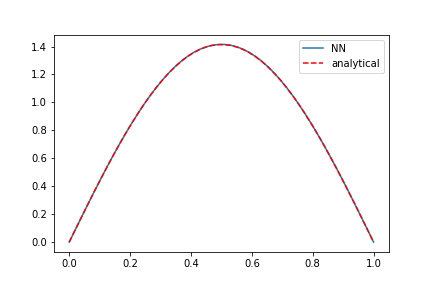
\includegraphics[width=3in,height=3in,keepaspectratio]{n1L1E5p5_plot.png}
    \label{fig:n1L1_plot}
    \caption{Wavefunction for n=1, L=1}
\end{figure}

\justify
It is matching very well with the analytical curve. This is marked by the final value of the MSE loss ($0.01044$) and the learned eigenvalue ($4.93483818$) which is accurate upto 4 places of decimal. The MSE loss can be further decreased to the order of $10^{-5}$ or lesser with 10,000 training epochs.

\justify
It is informative to check some diagnostic curves for this case. The \MSE \ vs. \iterations curve is below -

\begin{figure}[!htb]
    \centering
    \includegraphics[width=3.0in,height=3.0in,keepaspectratio]{n1L1E5p5_diagMSE.png}
    \label{fig:n1L1_MSE}
    \caption{MSE curve for n=1, L=1}
\end{figure}

\justify
The MSE loss quickly falls to zero in a few epochs. It is also helpful to observe the behaviour of other network parameters in diagnostic plots. The other two curves plotted below are that of \probability vs. \iterations and \eigenvalue vs. \iterations -

\begin{figure}[!htb]
    \centering
    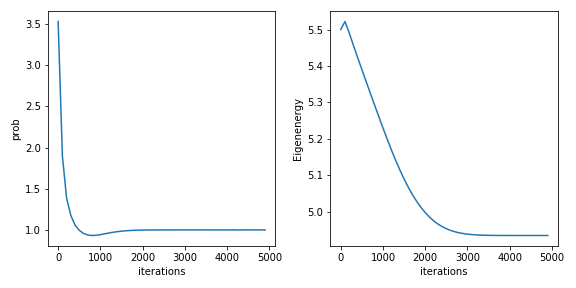
\includegraphics[width=5.0in,height=5.0in,keepaspectratio]{n1L1E5p5_diagProbEig.png}
    \label{fig:n2L3_probEig}
    \caption{Probability \& Eigenvalue curve for n=1, L=1}
\end{figure}

\justify
The probability needed a couple thousand of epochs to begin settling to 1. The eigenvalue also flattens to its correct value in a similar fashion.

\subsection{n=2, L=1}

\justify
The correct eigenvalue is $\displaystyle{2\pi^2} = 19.7392088$. Initialising the energy parameter E to $22$, the following plot is obtained - 

\begin{figure}[!htb]
    \centering
    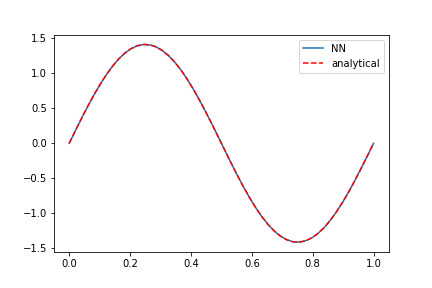
\includegraphics[width=3.0in,height=3.0in,keepaspectratio]{n2L1E23_plot.png}
    \label{fig:n2L1_plot}
    \caption{Flat Wavefunction for n=2, L=1}
\end{figure}

\justify
The network has learned a flat wavefunction. Although the MSE term is low ($0.0022$), the final probability obtained is vanishingly low at $1.4 \times 10^{-7}$. The eigenvalue learned is also incorrect at 22.967. The reason for this can gauged from the \probability vs. \iterations diagnostic curve below

\begin{figure}[!htb]
    \centering
    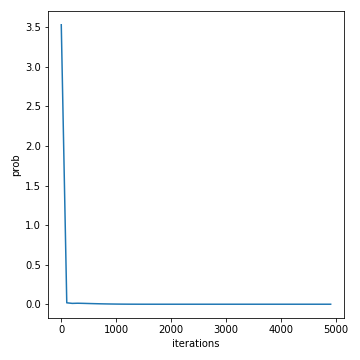
\includegraphics[width=3.0in,height=3.0in,keepaspectratio]{n2L1E23_diagProb.png}
    \label{fig:n2L1_diagProb}
    \caption{Probability curve for n=2, L=1}
\end{figure}

\justify
It isn't the case that the probability slowly falls to zero over the iterations. The probability plummets to zero immediately, and \textit{also} results in a flat wavefunction. In terms of optimization of the loss function, this makes sense as a flat wavefunction is a \textit{trivial} way to make the \MSE \ term vanish. A similar behaviour was noticed with other cases of $n$ and $L$ (\textit{especially for higher values of the ratio \nLratio}) and it was concluded that the network has a tendency to learn the \textit{trivial} solution.


\section{Probability Regularization}

\justify
A possible solution is to avoid the plummeting of the probability is to strengthen the loss function with regularization terms as function of probability p. Its purpose is two-fold -
\begin{enumerate}
    \item It would prevent the probability from hitting zero
    \item It would force the network to learn a \textit{non-trivial} eigenfunction and the correct eigenvalue
\end{enumerate}

\justify
A regularisation term of $\displaystyle{\frac{1}{p}}$ would force the probability away from 0, and there is no harm in doing so as $p \geq 0$ by construction. However, this would have the side-effect of pushing the probability beyond 1 as $\displaystyle{\frac{1}{p}}$ is a monotonically decreasing function of $p$. This can be counter-acted by linear or higher degree terms such as $p$ or $p^2$. 

\justify
As a generic case, the regularization function was chosen as follows -
$$\displaystyle{
R(p) = \frac{a}{p} + \frac{c}{p^2} + \frac{e}{p^3} + \frac{g}{p^4} + bp + dp^2 + fp^3 + hp^4
}$$

\justify
It needs to be ensured that the loss function has a local minima at $p=1$. The $(1-p)^2$ term already has a global minima at $p=1$. Hence, finding the derivative of $R$ with respect to $p$ is sufficient -
$$\displaystyle{\dv{R}{p} = -\frac{a}{p^2} - \frac{2c}{p^3} - \frac{3e}{p^4} - \frac{4g}{p^5} + b + 2dp + 3fp^2 + 4hp^3}$$

\justify
Setting this derivative 0 at $p=1$, we get -
$$\displaystyle{a + 2b + 3c + 4g = d + 2e + 3f + 4h}$$

\justify
It would be desired that in the neighbourhood of $p=1$, the dominating regularising terms are $\displaystyle{\frac{a}{p}}$ and $dp$ and not the other terms. The higher exponent terms will automatically dominate for a relatively larger value of $\left|p-1\right|$. Hence, we must ensure that  Thus, one can choose -
$$\displaystyle{
c =  \frac{a}{4} \ \text{,} \ e = \frac{c}{6} \ \text{,} \ g = \frac{e}{8}
}$$

\justify
and
$$\displaystyle{
d = \frac{b}{2} \ \text{,} \ f = \frac{d}{6} \ \text{,} \ h = \frac{f}{8}
}$$

\justify
If we denote $\displaystyle{\Delta p_a}$ as the change in the probability due to the $\displaystyle{\frac{a}{p}}$ term at $p=1$, and likewise for other terms, then the choice of co-efficients above ensures that -
$$\displaystyle{
\Delta p_a = 2\Delta p_c = 4\Delta p_e = 8\Delta_g \ \text{and} \ \Delta p_b = 2\Delta p_d = 4\Delta p_f = 8\Delta p_h
}
$$

\justify
Making an arbitrary choice of $a = d = 20$, the final regularisation function is -
$$\displaystyle{
R = \frac{20}{p} + \frac{5}{p^2} + \frac{5}{6p^3} + \frac{5}{48p^3} + 20p + 5p^2 + \frac{5p^3}{6} + \frac{5p^4}{48}
}$$

\justify
The condition $a + 2b + 3c + 4g = d + 2e + 3f + 4h$ is automatically satisfied by construction. Now the minimum value the loss function could attain is $\left(a+b+c+d+e+f+g+h\right)$ which turns out to be $51.875$ in our case. The MSE term could still attain a lowest possible value of 0, however. The plot of only the $p$ terms of the loss $L(p) = (1-p)^2 + R(p)$, and its derivative, is given below -

\begin{figure}[!htb]
    \centering
    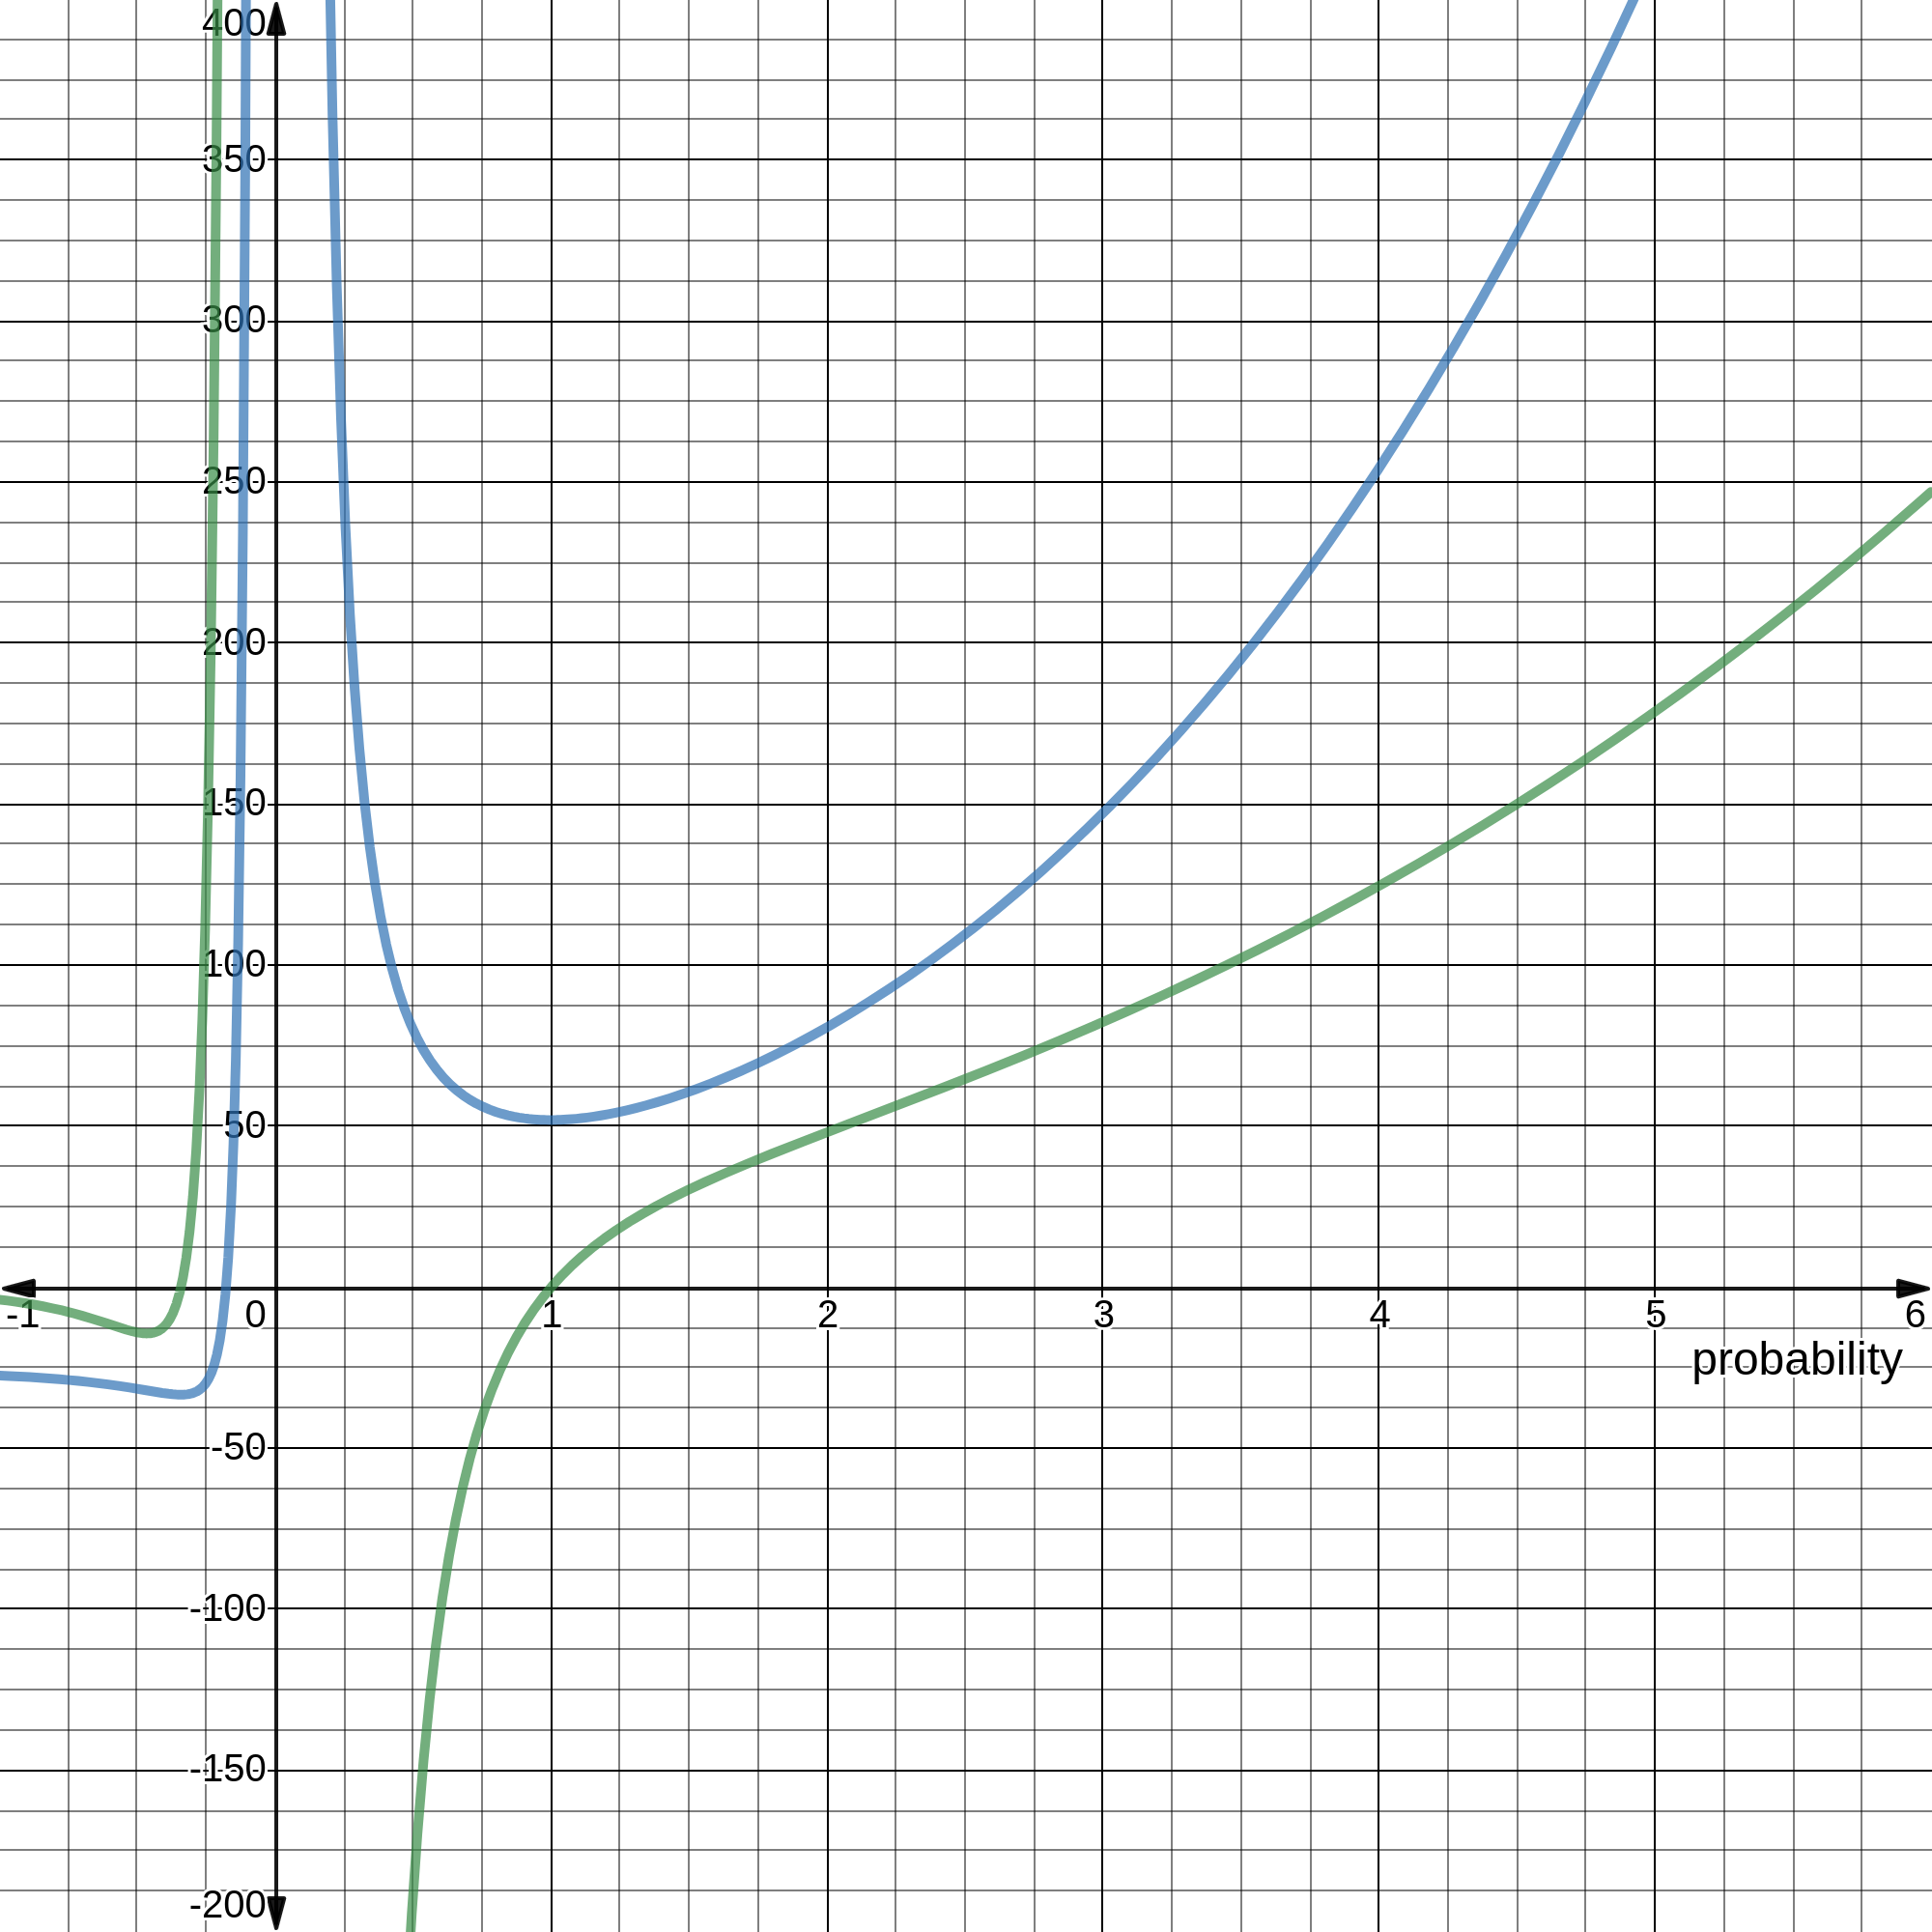
\includegraphics[width=5.5in,height=5.5in,keepaspectratio]{probReg.png}
    \label{fig:probReg}
    \caption{Probability Regularization graph}
    \subcaption{Blue : Regularization term, Green : Its derivative}
\end{figure}

\newpage

\justify
There is a strong derivative for $p<1$ to prevent the probability from falling to 0. At the same time, the derivative for $p>1$ is not as strong as to the left of it, which would work well for our purposes.

\subsection{n=2, L=1}

\justify
The above scheme of regularisation works extremely well for this case. The final value of the MSE loss is $0.00108643$, and the final probability is $1.0000119$. The eigenvalue learned is $19.73925203$ which is again correct upto 4 places of decimal. The wavefunction is given below - 

\begin{figure}[!htb]
    \centering
    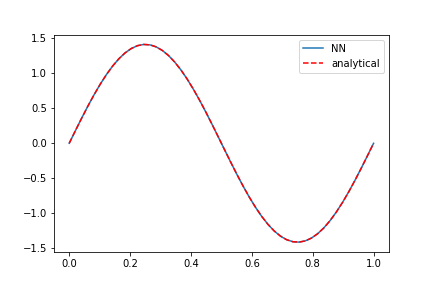
\includegraphics[width=3.0in,height=3.0in,keepaspectratio]{n2L1E23_plotReg.png}
    \label{fig:n2L3_plotReg}
    \caption{Wavefunction for n=2, L=1}
\end{figure}

\justify
The neural network learns the desired wavefunction. It is also interesting to look at the  \probability vs. \iterations curve to check the effect of the regularization terms - 

\begin{figure}[!htb]
    \centering
    \includegraphics[width=3.0in,height=3.0in,keepaspectratio]{n2L1E23_diagProbReg.png}
    \label{fig:n2L3_plotReg}
    \caption{Probability curve for n=2, L=1 after regularization}
\end{figure}

\justify
The initial behaviour of the probability is the same as in the previous case, however the regularization terms push the probability away from 0. It then grows upto 1 quickly and oscillates in a small neighbourhood about 1. In general it was observed, that for lower values of the ratio $\displaystyle{\frac{n}{L}}$, the regularisation works quickly. For higher values of the ratio, the probability approaches 1 slower. Hence, the number of training iterations cannot be fixed for every case and this very issue is discussed in the next section.

\subsection{n = 5, L = 2}

\justify
The true eigenvalue is $\displaystyle{\frac{5^2 \pi^2}{2 2^2}} = 30.8425137$ and the learned value is $30.84252368$ which is again correct upto 4 decimal places. The probability obtained is $0.997989$. The final MSE loss is $0.16477485$. This is higher than the previously obtained losses by 2 orders of magnitude, but this could be explained by two factors - 
\begin{enumerate}
    \item The wavefunction for n=5 has 5 extremas and a continuously changing curvature which is a source of error in the $\displaystyle{\dv[2]{\psitilde}{x}}$ term of the loss function
    \item Limited resolution of the training set over the range $\left[0,L\right]$, coupled with the normalization constraint introduces error in the probability density numerical integration.
\end{enumerate}

\begin{figure}[!htb]
    \centering
    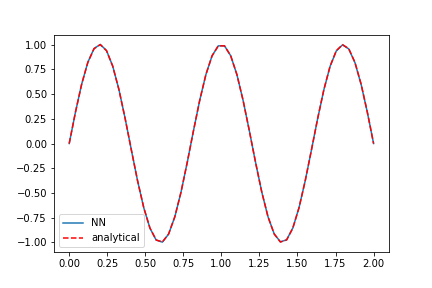
\includegraphics[width=3.0in,height=3.0in,keepaspectratio]{n5L2E35_plot.png}
    \label{fig:n5L2_plot}
    \caption{Wavefunction for for n=5, L=2}
\end{figure}

\justify
The diagnostic curves of \probability vs. \iterations and \eigenvalue vs. \iterations (Fig 11) are well-behaved too, although they stabilize slower than the previous case (\textbf{3.1}). They flatten to their stable values at approximately the same number of epochs simultaneously. It is desired that this simultaneous stabilization is observed across all cases as it would imply that the eigenfunction and eigenvalue enforce each other strongly through the derivatives of the loss. It is also desired that there is significant flattening over the last couple thousand epochs of the training as it would allow the eigenfunction and eigenvalue to obtain precision. 

\justify
In other cases, especially for higher ratios of $\displaystyle{\frac{n}{L}}$, the simultaneity of the probability and eigenvalue is not achieved strongly over the epochs. The probability reaches 1 too quickly and the eigenvalue fails to be trained, or it occurs that the eigenvalue is nearly accurate but the growth rate of the probability is too slow.

\newpage

\begin{figure}[!htb]
    \centering
    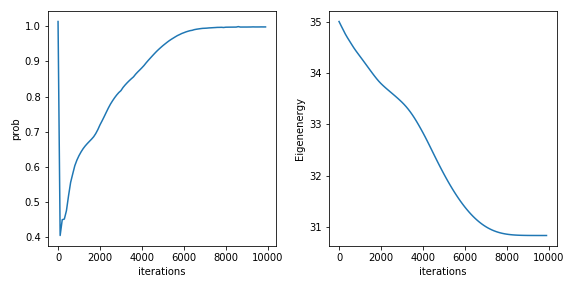
\includegraphics[width=5.0in,height=5.0in,keepaspectratio]{n5L2E35_diagProbEig.png}
    \label{fig:n5L2_diagProbEig}
    \caption{Probability and Eigenvalue curves for n=5, L=2}
\end{figure}

\section{Exit Conditions}

\justify
It is interesting to observe the case of $n = 7, L = 1$. This has a high ratio of \nLratio compared to any case seen previously. After training for 150,000 epochs, a loss of $0.04669563$ is obtained which is an order of magnitude higher than the previous cases, coupled with the large number of epochs. The wavefunction graph also has large granularity due to the limit of resolution on the real number line, which chokes the precision of all loss terms greatly. Also, the final probability is $0.99331093$ which only confirms this fact, and is an order magnitude lower in precision compared to previous cases. The eigenvalue, however, was learnt accurately as $241.80534101$ which is again precise upto 4 decimal places in comparison to $\displaystyle{\frac{49 \pi^2}{2} = 241.8053078}$


\begin{figure}[!htb]
    \centering
    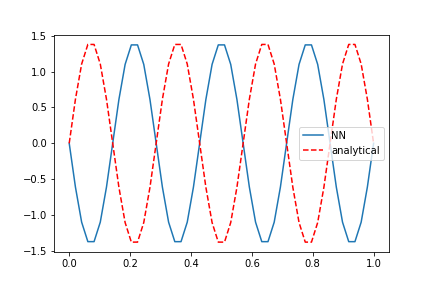
\includegraphics[width=3.0in,height=3.0in,keepaspectratio]{n7L1E260_plot.png}
    \label{fig:n5L2_diagProbEig}
    \caption{Wavefunction for n=7, L=1}
\end{figure}

\justify
It is natural to quit training once a desired level of precision is reached in the loss. The loss, in our case, has too many terms and hence its behaviour isn't reliable enough upon which to build an exit condition. Observing the behaviour of the MSE, probability, and eigenvalue terms over the training of many cases, the following observation could be made upon an exit condition to stop training -
\begin{enumerate}
    \item It is not sensible to fix the number of epochs to an extremely high number. For cases with small value of \nLratio, less than 10,000 epochs are sufficient to reach precisions of \oom{-6} in the MSE. Although there is no fear of \textit{overfitting} in this Machine Learning problem, it would lead to wastage of time.
    \item It wouldn't be advisable to increase the learning rate of the underlying optimization algorithm. Multiple local minima exist and the gradients must not overshoot.
    \item The exit condition cannot be depend upon the precision reached on the probability term (\textit{such as \oom{-3} or \oom{-4}}) due to the limit of resolution on the training set.
    \item It cannot depend upon the precision reached on the loss due to similar reasons, and for wavefunctions with continuously changing curvature - higher ratios of \nLratio. In some cases, the jump from \oom{-2} to \oom{-3} could take $20,000$ epochs, whereas the jump from \oom{-3} to \oom{-4} could take more than $100,000$
    \item Neither can it depend on the precision of the eigenvalue as it is a matter of scale of the problem, which we cannot judge \textit{a priori}.
    \item On the other hand, the \textit{difference} in the MSE every hundred epochs, \dmse, has proven to have reliable behaviour across all cases. At the end of training it has taken values in the order of $10^{-4}$ Logically, it is sensible to use this to decide the halting of the training due to the following reasons
    \begin{itemize}
        \item \dmse could reach a precision of \oom{-4} even at lower values of probability such as $0.98$ or $0.95$. It is not necessary that very high levels of precision in probability be reached before \dmse could enjoy high precision. Hence, it would take care of cases of high curvature and limited numerical resolution.
        \item When \dmse reaches a certain level of precision, it means that the limit of numerical resolution of the system has been reached. It would avoid any pitfalls created by point 1 above. In other words, it wouldn't matter if the MSE saturated at order of magnitude \oom{-1} or \oom{-3}. If the resolution is choked, the \dmse can only improves at a much lower precision, which has been chosen as \oom{-4}
        \item Exit conditions based on \dmse would handle cases where the training does not exhibit the simultaneous stabilization of the probability and the eigenvalue.
    \end{itemize}
\end{enumerate}

\justify
Having enlisted these observations, the \adam optimizer was modified with the use of \callback to take into account the exit conditions. The epoch at which \dmse reaches a value of \oom{-2} denotes the onset of precision of the network. This point could be reached before or after 10,000 epochs, which has been taken as a cutoff heuristically. Based on either case, two exit conditions have been designed - \lTTTExit (\textit{less than ten thousand}) and \normalExi, respectively . Also depending on the subsequent behaviour of the training, \lTTTExit could transition to \normalExit, however \normalExit doesn't transition when it's set at the onset of precision.

\subsection{Epoch Limits During Training}

\justify
As the training loop goes through its iterations, various epoch limits are set based on the precision of \dmse. \\

\begin{algorithm}[H]
\caption{\texttt{\textbf{Train\_setEpchLim}}}\label{alg:setEpchLim}
\begin{algorithmic}[1]
\State /* $i_2 \gets$ Epoch number at which \dmse hits \oom{-2} */
\State /* $lim_3 \gets $ Epoch limit before which \dmse should hit \oom{-3} */
\State /* $i_3 \gets$ Epoch number at which \dmse hits \oom{-3} */
\State /* $lim_4 \gets $ Epoch limit before which \dmse should hit \oom{-3} */
\State /* $i_4 \gets$ Epoch number at which \dmse hits \oom{-4} */
\State /* $endlim \gets $ Epoch limit before which \dmse should hit \oom{-4} 5 times */
\State /* $count \gets $ No. of times \dmse has hit \oom{-4} or below */

\State Initialise $i_2, lim_3, i_3, lim_4, i_4, endlim$ to \textit{NULL} 
\State Initialise $count, epch$ to 0

\While {True}
    \State $epch \gets epch + 1$
    \State /* Perform training */
    \If{\dmse hits \oom{-2}}
        \State $i_2 \gets $ epch
        \State $lim_3 \gets 2i_2$ 
    \EndIf

    \If{\dmse hits \oom{-3}}
        \State $i_3 \gets epch$ 
        \If{$i_3 + 4(i_3-i_2) > 2i_3$}
            \State $lim_4 \gets 2i_3$
\algstore{setEpchLim}
\end{algorithmic}
\end{algorithm}

\begin{algorithm}[H]
\caption{\texttt{\textbf{Train\_setEpchLim}} (Continued)}\label{alg:setEpchLim}
\begin{algorithmic}[1]
\algrestore{setEpchLim}
        \ElsIf{$\displaystyle{\ceil*{\frac{3i_3}{2}} < i_3 + 4(i_3-i_2) < 2i_3}$}
            \State $lim_4 \gets i_3 + 4(i_3-i_2)$
        \Else
            \State $\displaystyle{lim_4 \gets \ceil*{\frac{3i_3}{2}}}$
        \EndIf
        
        \If{$lim_4 < lim_3$}
            \State $lim_4 \gets 2lim_3 - lim_4$
        \EndIf
    \EndIf
    
    \If{\dmse hits \oom{-4}}
    \State $count \gets count + 1$
    \State $i_4 \gets epch$ 
    \If{$i_4 + 8(i_3-i_2) > 2i_4$}
        \State $endlim \gets 2i_4$
    \ElsIf{$\displaystyle{\ceil*{\frac{3i_4}{2}} < i_4 + 8(i_4-i_3) < 2i_4}$}
            \State $endlim \gets i_4 + 8(i_4-i_3)$
        \Else
            \State $\displaystyle{endlim \gets \ceil*{\frac{3i_4}{2}}}$
        \EndIf
        
        \If{$endlim < lim_4$}
            \State $endlim \gets 2lim_4 - endlim$
        \EndIf
    \EndIf
    
    \begin{comment}
    \If{$i_4$ \textbf{is not} \textit{NULL}}
        \If{$\left(count < 5 \ \textbf{and} \ epch > endlim\right) \ \textbf{or} \ count \geq 5$}
            \State \textbf{break}
        \EndIf
    \EndIf
     \If{$i_3$ \textbf{is not} \textit{NULL} \textbf{and} $epch < lim_4$}
        \State \textbf{break}
    \EndIf
    \If{$i_2$ \textbf{is not} \textit{NULL} \textbf{and} $epch < lim_3$}
        \State \textbf{break}
    \EndIf
    \end{comment}
    
_    \If{$i2 > 10,000$}
        \State \textbf{call} \normalExit
    \Else
        \State \textbf{call} \lTTTExit
    \EndIf
\EndWhile
\end{algorithmic}
\end{algorithm}

\subsection{\texttt{NormalExit}}

\justify
This exit condition will be used when \dmse reaches \oom{-2} for the first time after 10,000 iterations. In this case, the training will exit when \dmse holds a value of \oom{-4} atleast 5 times, or any of the three limiting epochs are reached.

\begin{algorithm}[H]
\caption{\normalExit}\label{alg:normalExit}
\begin{algorithmic}[1]
\If{$i_4$ \textbf{is not} \textit{NULL}}
    \If{$\left(count < 5 \ \textbf{and} \ epch > endlim\right) \ \textbf{or} \ count \geq 5$}
        \State \textbf{break}
    \EndIf
\algstore{normalExit}
\end{algorithmic}
\end{algorithm}

\begin{algorithm}[H]
\caption{\normalExit (Continued)}\label{alg:normalExit}
\begin{algorithmic}[1]
\algrestore{normalExit}
\EndIf
\If{$i_3$ \textbf{is not} \textit{NULL} \textbf{and} $epch > lim_4$}
    \State \textbf{break}
\EndIf
\If{$i_2$ \textbf{is not} \textit{NULL} \textbf{and} $epch > lim_3$}
    \State \textbf{break}
\EndIf
\end{algorithmic}
\end{algorithm}

\subsection{\texttt{L3TExit}}

\justify
In this case, the training will exit when \dmse holds a value of \oom{-4} atleast 10 times, or it decides to switch to \normalExit after checking any of the limiting epochs with a threshold of $20,000$.

\begin{algorithm}[H]
\caption{\lTTTExit}\label{alg:lTTTExit}
\begin{algorithmic}[1]
\If{$i_3$ \textbf{is not} \textit{NULL} \textbf{and} $lim_4 > 20,000$}
    \State \textbf{call} \normalExit
\EndIf
\If{$i_4$ \textbf{is not} \textit{NULL}}
    \If{$endlim > 20,000$}
        \State \textbf{call} \normalExit
    \ElsIf{$count >= 10$}
        \State \textbf{break}
    \EndIf
\EndIf
\end{algorithmic}
\end{algorithm}

\subsection {n = 7, L = 1}

\begin{figure}[!htb]
    \centering
    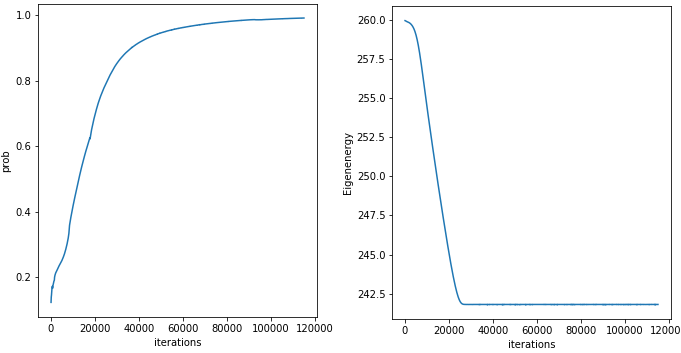
\includegraphics[width=4.5in,height=4.5in,keepaspectratio]{n7L1E260_gimp.png}
    \label{fig:n7L1_diagGimp}
    \caption{Wavefunction for n=7, L=1}
\end{figure}

\justify
When \adam with the exit conditions was run on this case, it needed a total of 111,000 epochs. Thus, 40,000 epochs were saved from the previous run with negligible difference in precision. The eigenvalue reported as the same precision, and the loss is $0.043613$ which is infact slightly better than the previous run with 150,000 epochs. The probability is also $0.990647$.

\justify
The exit conditions have allowed the probability enough epochs to settle whilst not overtraining the network. It is also interesting to observe how the eigenvalue settles around epoch 25,000 whereas the probability reaches precisions of \oom{-1} only above epoch 100,000. This is a clear sign of the limited numerical resolution of the system.


\section{Eigenvalue Regularization}

\justify
The only control over the energy parameter is its initialization. The user of the network has no say over the eigenvalue the network will learn, as there are many of them. It would be desirable to restrict the search of the eigenvalue within a certain range. This could be achieved, again, by regularization terms.

\subsection{Derivation}

\justify
The scale of the problem is defined by the range $\left[E_1, E_2\right]$ to search the eigenvalue in. It can easily be captured by the number $m = \log_{10}(E_2 - E_1)$. Consider a regularization function $f(E)$ -
$$\displaystyle{
f(E) = \frac{1}{k} \left[
\frac{1}{(E-r_1)^n} + \frac{1}{(E-r_2)^n}
\right]
}$$

\justify
Its derivative is -
$$\displaystyle{
f'(E) = -\frac{n}{k} \left[
\frac{1}{(E-r_1)^{n+1}} + \frac{1}{(E-r_2)^{n+1}}
\right]
}$$

\justify
$r_1$ and $r_2$ define singularity points and asserting that $E_1 = r_1 + \epsilon_1$ and $E_2 = r_2 - \epsilon_2$, where the neural network would search the energy parameter. Since the learning rate of \adam is \oom{-3}, we can set the following to keep our derivatives small at the limits -
$$\displaystyle{
10^{-3} \left| f'(E_1) \right| < 10^{m-4}
\ \ \text{and} \ \ 
10^{-3} \left| f'(E_2) \right| < 10^{m-4}
}
$$

\justify
When the derivative is fixed in such manner, it ensures that the contribution to $\Delta E$ due to regularization is small in the middle of the range $\left[E_1,E_2\right]$, where the neural network is expected to find a stable eigenvalue. It's undesirable for this stability to be disturbed due to the above terms. It is also necessary to have a strong derivative near the singularities to contain the eigenvalue within the range. Using the first condition, we get -
$$\displaystyle{
\left|-\frac{n}{k} \left[
\frac{1}{(\epsilon_1)^{n+1}} + \frac{1}{(r_1-r_2+\epsilon_1)^{n+1}}
\right]\right| < 10^{m-1}
}
$$

\justify
which gives -
$$\displaystyle{
\left[
\frac{1}{(\epsilon_1)^{n+1}} + \frac{1}{(r_1-r_2+\epsilon_1)^{n+1}}
\right] < \frac{10^{m-1}k}{n}
}
$$

\justify
The second term on the LHS can be ignored as $\left|r_1 - r_2\right| >> \epsilon_1$. In particular, we can choose $n=8$ and state that $n \sim 10^{1}$ which gives -
$$\displaystyle{
\epsilon_1^{-\left(n+1\right)} < 10^{m-2}k \implies \epsilon_1 < \left(10^{m-2}k\right)^{-\frac{1}{n+1}}
}
$$

\justify
Since $\epsilon_1$ is the distance between an eigenvalue limit and the singularity, we can choose that $\epsilon_1 < 10^{m-2}$. Taking $k$ of the form \oom{s}, we can equate the RHS of the above two inequalities -
$$\displaystyle{
\left(10^{m-2+s}\right)^{-\frac{1}{n+1}} = 10^{m-2} \implies s = (2 - m)(n + 2)
}$$

\begin{figure}[!htb]
    \centering
    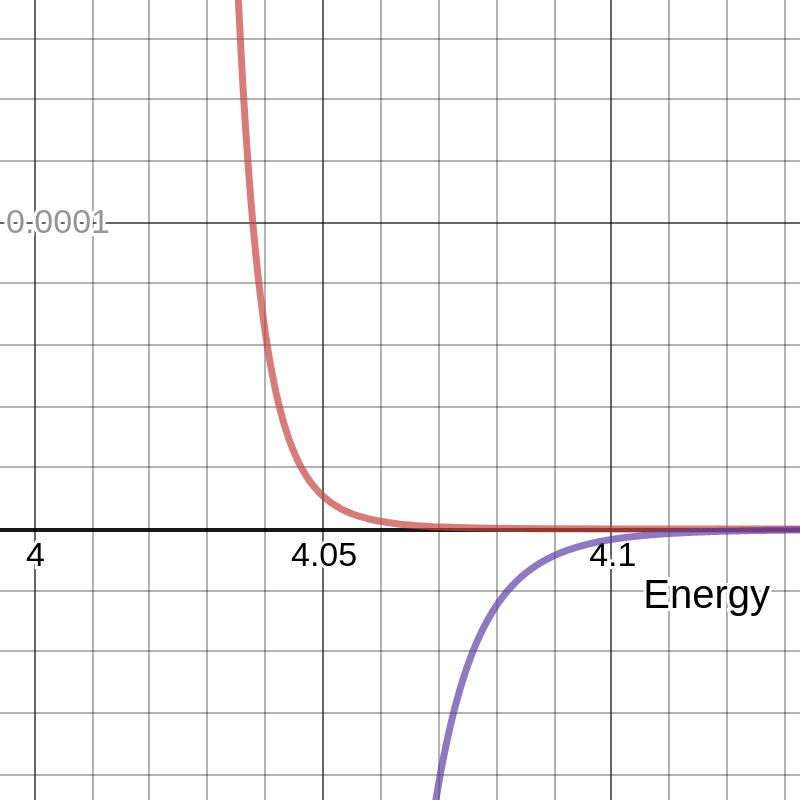
\includegraphics[width=3.0in,height=3.0in,keepaspectratio]{Ereg.png}
    \label{fig:Ereg}
    \caption{Eigenvalue Regularization Graph}
    \subcaption{Red : $f(E)$, Purple : $f'(E)$}
\end{figure}

\justify
Note how quickly the function flattens for the case $E_1 = 4, E_2 = 8$. The same behaviour is observed near $E=8$ as well. The derivative grows faster than the function near the singularity.

\subsection{E1 = 2.5, E0 = 3.25, E2 = 4}

\justify
Firstly, it is helpful to observe the results without eigenvalue regularization. Consider case of $L=4$. The following is the \eigenvalue vs. \iterations plot without controlling the eigenvalue regularization -

\begin{figure}[!htb]
    \centering
    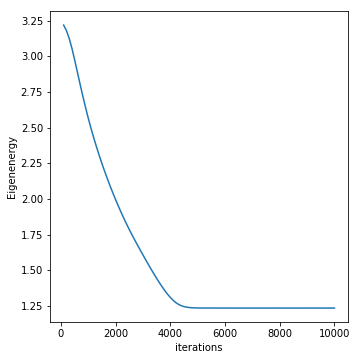
\includegraphics[width=3.0in,height=3.0in,keepaspectratio]{Ereg_fallThrough.png}
    \label{fig:Ereg_fallThrough}
    \caption{Eigenvalue Falling Through}
\end{figure}

\justify
The network falls down below $E_1 = 2.5$ and learns the eigenvalue for the $n=2$ case. Now, with the eigenvalue regularization terms added, the plot changes as follows -
\begin{figure}[!htb]
    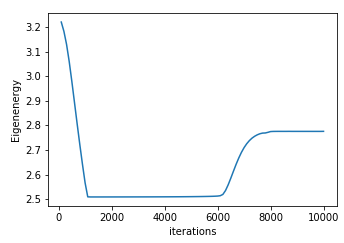
\includegraphics[width=3.0in,height=3.0in,keepaspectratio]{Ereg_eflat.png}
    \label{fig:Ereg_stable}
    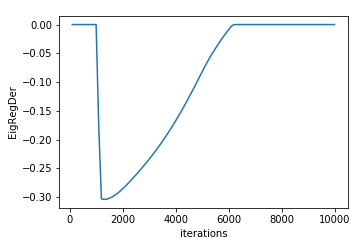
\includegraphics[width=3.0in,height=3.0in,keepaspectratio]{Ereg_eder.png}
    \label{fig:Ereg_der}
    \caption{Plots of eigenvalue and its regularization derivative}
\end{figure}

\justify
It is clear how an increase in magnitude of the regularization derivative forces the eigenvalue to go up from $2.5$ an stabilize at the energy level for $n=3$ (2.77).

\subsection{E1 = 2, E0 = 2.2, E2 = 3}

\begin{figure}[!htb]
    \centering
    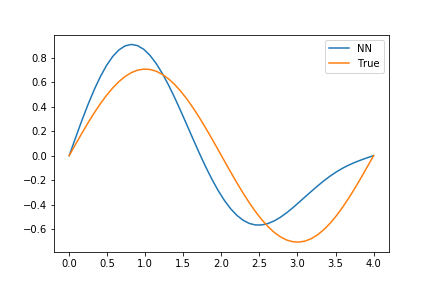
\includegraphics[width=3.0in,height=3.0in,keepaspectratio]{L4E2E2p2E3_plot.png}
    \label{fig:Ereg_fallThrough}
    \caption{Wavefunction with premature shape}
\end{figure}

\justify
There is a significant difference between the network's output and the analytical answer. The eigenvalue learnt by network is $2.00536509$ which does not correspond to any $E_n$ for $L=4$. For $n=2$, $E_2 = 1.2337005$ and for $n=3, E_3 = 2.775826$. It was hoped that the eigenvalue regularization would push the network back up to learn $E_3$ although it had a tendency to fall towards $E_2$. Although the probability is good $0.99845$, the MSE is $0.14805912$ which is unsatisfactory for this case of low \nLratio. Further insight can be obtained by looking at the curve of the eigenvalue regularization derivative.

\begin{figure}[!htb]
    \centering
    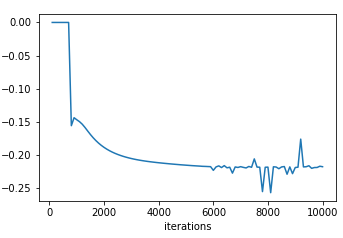
\includegraphics[width=3.0in,height=3.0in,keepaspectratio]{Ereg_ederNonZero.png}
    \label{fig:Ereg_fallThrough}
    \caption{Eigenvalue Regularization Derivative}
\end{figure}

\justify
In the previous case, the regularization derivative flattens to zero over the final epochs. However, for the present case the derivative is still trying to push back the eigenvalue inside the range. This explains why the learnt eigenvalue didn't correspond to any $E_n$


\section{Improvements}

\justify
In this report, attempts have been made to generalise the neural network over multiple cases. However, it is noted that for particular cases the training is slower than others. This could be fixed by normalizing the differential equation for any value of $L$ and then solving the system.

\justify
Currently, the entire training set is considered at once to optimize the loss, which slows down training over the epochs. This was deemed as necessary because the probability density integral needed to be calculated. However, it is possible to train the network in batches and perform the optimization. Currently $tanh$ activation is used, but it suffers from the vanishing gradient. Other activations could be looked into.

\justify
It is possible to conceive of an architecture of two simultaneous neural networks - \textit{one for the eigenfunction, and the other for the eigenvalue} - that is trained over a common loss function. It has been noticed that the eigenvalue changes in similar magnitudes irrespective of the scale of the system (L), which is clearly a problem. This could be overcome by having a separate neural network output the eigenvalue. In some sense, the nodes backing the eigenvalue output offers more control over its change, and it could dynamically take care of the scale of the problem. In the case of eigenvalue regularization, \adam could be modified to externally increase eigenvalue derivative dynamically if it is noticed that it has spent many too many epochs near either of the singularity points. 

\justify
Pertinent issues -
\begin{enumerate}
    \item The choice of the energy parameter initialisation seems back-engineered and specific to the problem. Having a separate neural network control the eigenvalue output could fix the issue. Also it could well be extended to a generic Quantum Mechanics problem.

    \item The decision of using \dmse for the exit condition could again be attributed to specificity. It seemed natural only \textit{after} manually observing the training of multiple cases. It may not apply from all differential equations or potentials.
    
    \item Due to the lack of control in the eigenvalue derivatives, it could be possible that it crosses any of singularities of the regularization terms, or lands exactly on it. There is no recovery from this situation in the present framework.
        \begin{enumerate}
            \item On a second thought, it could be possible to create infinite \textit{\"wells\"} of regularization terms such as $\displaystyle{\frac{1}{(E-E_1)^n} + \frac{1}{(E-E_2)^n} + \frac{1}{(E-E_3)^n} + \frac{1}{(E-E_4)^n}}$ \\
            
            \begin{itemize}
                \item This defeats the purpose of using regularization terms at all as the eigenvalue is free to assume any value. However, this could be a fruitful idea in the case of an unknown potential, whose eigenvalues are sought. It serve as a systematic way to divide the eigenvalue space and search for possible eigenfunction in them.
            \end{itemize}
            \item Gradient clipping on the eigenvalue could be done near the singularity points to prevent the jump
             \item It is difficult to judge if the network has learnt the correct wavefunction or not. However, this could be solved by observing the eigenvalue regularization derivatives near the end of the training.
        \end{enumerate}
        
    \item Particle in a Box is further simplified by the fact that the potential is infinity outside the box. We know \textit{a priori} that the wavefunction vanishes in such regions. However, for the generic potential, the square integrability of the wavefunction has to be checked for $x \xrightarrow{} \pm \infty$. Using any numerical integration technique for the entire position space could slow down the training immensely.
\end{enumerate}

\end{document}
